\documentclass{article}

\usepackage{fancyhdr}
\usepackage{extramarks}
\usepackage{amsmath}
\usepackage{amssymb}
\usepackage{enumerate}
\usepackage{graphicx}
\usepackage{braket}
\usepackage{cancel}
\usepackage{pgfplotstable}
\usepackage{listings}

\lstset{framexleftmargin=5mm, frame=shadowbox, rulesepcolor=\color{blue}}

% Useful things
\newcommand{\vcenteredinclude}[1]{\begingroup
\setbox0=\hbox{\includegraphics{#1}}%
\parbox{\wd0}{\box0}\endgroup}

%% better: (general command to vertically center horizontal material)
\newcommand*{\vcenteredhbox}[1]{\begingroup
\setbox0=\hbox{#1}\parbox{\wd0}{\box0}\endgroup}

%
% Basic Document Settings
%

\topmargin=-0.45in
\evensidemargin=0in
\oddsidemargin=0in
\textwidth=6.5in
\textheight=9.0in
\headsep=0.25in

\linespread{1.1}

\pagestyle{fancy}
\lhead{\hmwkAuthorName}
\chead{\hmwkClass\ : \hmwkTitle}
\rhead{\firstxmark}
\lfoot{\lastxmark}
\cfoot{\thepage}

\renewcommand\headrulewidth{0.4pt}
\renewcommand\footrulewidth{0.4pt}

\setlength\parindent{24pt}

%
% Create Problem Sections
%

\newcommand{\enterProblemHeader}[1]{
    \nobreak\extramarks{}{Problem \arabic{#1} continued on next page\ldots}\nobreak{}
    \nobreak\extramarks{Problem \arabic{#1} (continued)}{Problem \arabic{#1} continued on next page\ldots}\nobreak{}
}

\newcommand{\exitProblemHeader}[1]{
    \nobreak\extramarks{Problem \arabic{#1} (continued)}{Problem \arabic{#1} continued on next page\ldots}\nobreak{}
    \stepcounter{#1}
    \nobreak\extramarks{Problem \arabic{#1}}{}\nobreak{}
}

\setcounter{secnumdepth}{0}
\newcounter{partCounter}
\newcounter{homeworkProblemCounter}
\setcounter{homeworkProblemCounter}{1}
\nobreak\extramarks{Problem \arabic{homeworkProblemCounter}}{}\nobreak{}

%
% Homework Problem Environment
%
% This environment takes an optional argument. When given, it will adjust the
% problem counter. This is useful for when the problems given for your
% assignment aren't sequential. See the last 3 problems of this template for an
% example.
%
\newenvironment{homeworkProblem}[1][-1]{
    \ifnum#1>0
        \setcounter{homeworkProblemCounter}{#1}
    \fi
    \section{Problem \arabic{homeworkProblemCounter}}
    \setcounter{partCounter}{1}
    \enterProblemHeader{homeworkProblemCounter}
}{
    \exitProblemHeader{homeworkProblemCounter}
}

%
% Homework Details
%   - Title
%   - Due date
%   - Class
%   - Section/Time
%   - Instructor
%   - Author
%

\newcommand{\hmwkTitle}{Homework\ \#9}
\newcommand{\hmwkDueDate}{April 13, 2015}
\newcommand{\hmwkClass}{PHYS 5243 - Solid State Physics}
\newcommand{\hmwkClassInstructor}{Professor Sheena Murphy}
\newcommand{\hmwkAuthorName}{Chase Brown}


\begin{document}
	\begin{homeworkProblem}
		\textbf{Simon - Solid State Basics - Chapter 17, Problem 1: Holes}
		\\
		\begin{enumerate}[a)]
			\item In semiconductor physics, what is meant by a hole and why is it useful?
			\item An electron near the top of the valence band in a semiconductor has energy
				\begin{equation*}
					E = -10^{-37}|\textbf{k}|^2
				\end{equation*}
			where $E$ is in Joules and \textbf{k} is in $m^{-1}$. An electron is removed from a state $\textbf{k} = 2\times10^8 \text{m}^{-1} \hat{x}$, where $\hat{x}$ is the unit vector in the $x$-direction. For a hole, calculate (and give the sign of):
			\begin{enumerate}[(i)]
				\item the effective mass
				\item the energy
				\item the momentum
				\item the velocity
			\end{enumerate}
			\item If there is a density $\rho = 10^5 m^{-3}$ of holes, having almost exactly this same momentum, calculate the current density and it's sign. 
		\end{enumerate}
		\textbf{Solution}
		\\
		\begin{enumerate}[a)]
			\item A hole is the abscence of an electron where and electron would be found in the ground state of a lattice, atom, or molecue  It is useful in calculations to understand the properties of the hole, as electrons at the top of a valence band act as if they have negative mass.  Treating the absent electron as a hole returns the hole properties to positive mass.
			\item We are given the momentum vector and the energy of the electron:
				\begin{equation*}
					E_e = -10^{-37}|\textbf{k}|^2
				\end{equation*}
				\begin{equation*}
					\textbf{k} = 2\times10^8 \text{m}^{-1} \hat{x}
				\end{equation*}
				In Kittel Chapter 8 we are given the following relations for holes:
				\begin{equation*}
					\textbf{k}_h = -\textbf{k}_e 
				\end{equation*}
				\begin{equation*}
					\epsilon_h(\textbf{k}_h) = -\epsilon_e(\textbf{k}_e)
				\end{equation*}
				\begin{equation*}
					\textbf{v}_h = -\textbf{v}_e 
				\end{equation*}
				\begin{equation*}
					m_h = -m_e 
				\end{equation*}
				Therefore, we can calculate the following:
				\begin{enumerate}[(i)]
					\item 
						\begin{equation*}
							m^*_h = -\frac{\hbar^2|\textbf{k}|^2}{2(-10^{-37}|\textbf{k}|^2 \text{Joules})} = \frac{(6.625\times10^{-34} \text{Joules seconds})^2}{2(10^{-37} \text{Joules m}^2)} = 2.2\times10^{-30} \text{kg} = \boxed{2.41 m_e = m_h^*}
						\end{equation*} 
					\item 				
						\begin{equation*}
							E_h = -E_e = 10^{-37}|\textbf{k}|^2 = 10^{-37}|2\times10^8 \text{m}^{-1} \hat{x}|^2 \text{Joule m}^2 = 4\times10^{-21} \text{J} = \boxed{25 \text{meV} = E_h}
						\end{equation*}
					\item 						
						\begin{equation*}
							\textbf{p}_h = -\textbf{p}_e = -\hbar(2\times10^8 \text{m}^{-1} \hat{x}) = -2.1\times10^{-26} \frac{\text{m kg}}{\text{s}} \hat{x} = \boxed{\textbf{p}_h = -39.3 \frac{\text{eV}}{\text{c}}}
						\end{equation*}
					\item 
						\begin{equation*}
							\textbf{v}_h = -\textbf{v}_e = -\frac{\hbar(2\times10^8 \text{m}^{-1} \hat{x})}{m^*_h} = \boxed{-9587 \frac{\text{m}}{\text{s}}}
						\end{equation*}
				\end{enumerate}

				\item $\rho = 10^5 m^{-3}$
					\begin{equation}
						j = \textbf{v}_h*\rho = -9587 \frac{\text{m}}{\text{s}}10^5 m^{-3} = \boxed{9.6 \times 10^8\frac{\text{holes}}{m^2s}}
					\end{equation}
		\end{enumerate}
		
	\end{homeworkProblem}
	

	\pagebreak

	\begin{homeworkProblem}
		\textbf{Simon - Solid State Basics - Chapter 17, Problem 2: Law of Mass Action and Doping of Semiconductors}
		\\
		\begin{enumerate}[a)]
			\item Assume the band gap is much greater than the temperature ($E_g >> k_bT$).  Show that in a pure semiconductor at a fixed $T$, the product of the number of electrons ($n$) and the number of holes ($p$) depends only on the density of states in the conduction band and the density of dates in the valence band (through their effective mass), and on the band-gap energy.\\
			
			\begin{itemize}
				\item Derive expressions for $n$ and $p$ and for the product $np$. You may need to use the integral $\int_0^\infty \sqrt{x} e^{-x}dx = \frac{\pi}{2}$
			\end{itemize}
			
			\item The band gaps of Silicon and Germanium are 1.1 eV and 0.75 eV respectively.  You may assume the effective masses for silicon and germanium are isotropic, roughly the same, and are roughly 0.5 of the bare elctron mass for both electrons and holes. (Actually the effective masses are not quite the same, and furthermore the effective masses are both rather aniostropic, but we are just making a rough estimate here.)\\
			\begin{itemize}
				\item Estimate the conduction electron concentration for intrisic (undoped) silicon at room temperature.
				\item Make a rough estimate of the maximum concentration of ionized impurities that will still  allow for this "intrinsic" behavior.
				\item Estimate the conduction electron concentration for germanium at room temperature.
			\end{itemize}
		\end{enumerate}

		\textbf{Solution}
		\\
		\begin{enumerate}[a)]
			\item Equations for $n(T)$ and $p(T)$ are given in Simon - equations 17.8 and 17.9:
				\begin{equation*}
					n(T) = \frac{1}{4}\bigg(\frac{2m_e^*k_BT}{\pi\hbar^2}\bigg)^{\frac{3}{2}}e^{-\beta(\epsilon_c-\mu)}
				\end{equation*}
				\begin{equation*}
					p(T) = \frac{1}{4}\bigg(\frac{2m_h^*k_BT}{\pi\hbar^2}\bigg)^{\frac{3}{2}}e^{-\beta(\mu-\epsilon_v)}
				\end{equation*}
				and $n(T)p(T)$ is given by equation 17.10:
				\begin{equation*}
					n(T)p(T) = \frac{1}{2}\bigg(\frac{k_BT}{\pi\hbar^2}\bigg)^{3}\bigg(m_e^*m_h^*\bigg)^{\frac{3}{2}}e^{-\beta E_g}
				\end{equation*}
			\item $E_{g, Si} = 1.1$ eV, $E_{g, Ge} = 0.75$ eV, $m_e^* =m_h^*= 0.5m_e$:
				\begin{itemize}
					\item 
						\begin{equation}
							n(T)p(T) = \frac{1}{2}\bigg(\frac{k_BT}{\pi\hbar^2}\bigg)^{3}\bigg(m_e^*m_h^*\bigg)^{\frac{3}{2}}e^{-\beta E_g}
						\end{equation}
						We know that $n(T) = p(T)\Rightarrow n(T)p(T)=n(T)^2$ as this is an undoped crystal.
						\begin{equation}
							n(T)^2 = \frac{1}{2}\bigg(\frac{k_BT}{\pi\hbar^2}\bigg)^{3}\bigg(m_e^*m_h^*\bigg)^{\frac{3}{2}}e^{-\beta E_g}
						\end{equation}
						\begin{equation}
							n(T)_{Si} = \sqrt{\frac{1}{2}\bigg(\frac{k_BT}{\pi\hbar^2}\bigg)^{3}\bigg(0.5^2 m_e^2\bigg)^{\frac{3}{2}}e^{-\frac{1.1\text{eV}}{k_B(300K)}}} \Rightarrow \boxed{n(T)_{Si} = 0.00511 \frac{\text{electrons}}{\mu m^3}}
						\end{equation}

					\item In order to retain intrinsic properties, the doping must remain lower than a certain threshold reffered to as $I=n_{\text{instrinsic}}=p_{\text{instrinsic}}$.  
					\begin{equation}
						\boxed{n = \frac{1}{2}(\sqrt{D^2+4I}+D)}
					\end{equation}
					\item 						\begin{equation}
							n(T)_{Ge} = \sqrt{\frac{1}{2}\bigg(\frac{k_BT}{\pi\hbar^2}\bigg)^{3}\bigg(0.5^2 m_e^2\bigg)^{\frac{3}{2}}e^{-\frac{0.75\text{eV}}{k_B(300K)}}} \Rightarrow \boxed{n(T)_{Ge} = 4.475 \frac{\text{electrons}}{\mu m^3}}
						\end{equation}
				\end{itemize}
		\end{enumerate}
	\end{homeworkProblem}

	\pagebreak

\begin{homeworkProblem}
		\textbf{Simon - Solid State Basics - Chapter 17, Problem 3: Chemical Potential}
		\\
		\begin{enumerate}[a)]
			\item Show that the chemical potential in an intrinsic semiconductor lies in the middle of the gap at low temperature.
			\item Explain how the chemical potential varies with temperature if the semiconductor is doped with (i) donors (ii) acceptors.
			\item A direct-gap semiconductor is doped to produce a density of $10^{23} \frac{\text{electrons}}{m^3}$. Calculate the hole density at room temperature given that the gap is 1.0 eV, and the effective mass of carriers in the conduction and valence band are 0.25 and 0.4 electron mass respectively. Hint: use the result of Excercise 17.2a.
		\end{enumerate}
		\textbf{Solution}
		\\
		\begin{enumerate}[a)]
			\item The Fermi level (chemical potential) of a semiconductor lies at the middle of the band gap as there are electrons which fill the valence states, and the conduction band is empty under non doped and low temperature conditions.  From equation 17.11 in Simon we have:
				\begin{equation}
					\mu = \frac{1}{2}(\epsilon_c-\epsilon_v) + \frac{3}{4}(k_BT)log(\frac{m_h^*}{m_e^*})
				\end{equation}
				at $T=0$ we have
				\begin{equation}
					\mu = \frac{1}{2}(\epsilon_c-\epsilon_v) = \frac{1}{2}E_g
				\end{equation}
				
			\item 
				\begin{enumerate}[i)]
					\item For p-type doped semiconductors, the chemical potential lies closer to or below the valence band, and therefore as the temperature increases the electrons are excited to higher valence band states, and then (if the thermal energy is higher than the band gap and the lowered chemical pottential) across the band gap to the conduction band.
					\item For n-type doped semiconductors, the chemical potential lies closer to or above the conduction band, and therefore as the temperature increases the electrons are excited to higher conduction band states.
					
					This Fermi level shifting can be seen in the band structure below:\\
					\centerline{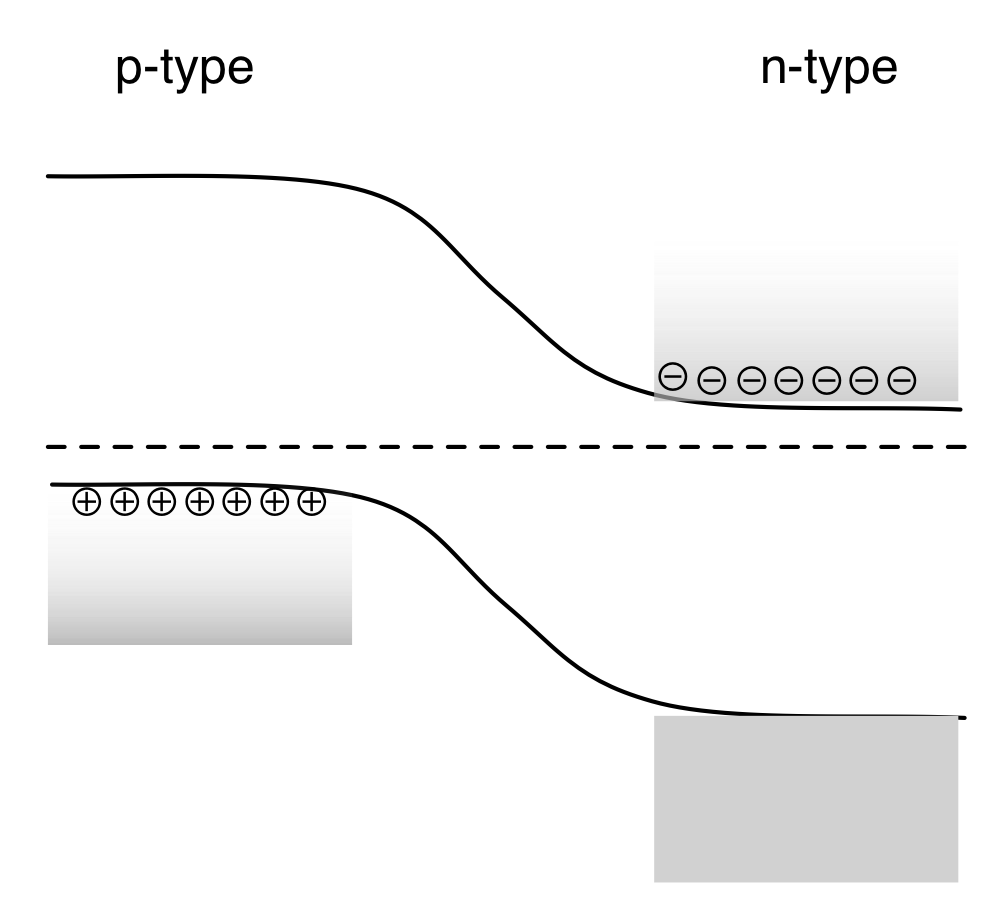
\includegraphics[scale=0.5]{pn.png}}
				\end{enumerate}
			\item The electron density is $n(T)=10^{23}\frac{\text{electrons}}{m^3}$ and the hole density is $p(T)$ at $RT=300K$ with $E_g=1.0$ eV, the effective masses are $m_e^* = 0.25m_e$ and $m_h^* = 0.4m_e$.  Therefore:
				\begin{equation*}
					n(T)p(T) = \frac{1}{2}\bigg(\frac{k_BT}{\pi\hbar^2}\bigg)^{3}\bigg(m_e^*m_h^*\bigg)^{\frac{3}{2}}e^{-\beta E_g}
				\end{equation*}
				\begin{equation}
					p(T) = \frac{1}{2n(T)}\bigg(\frac{k_BT}{\pi\hbar^2}\bigg)^{3}\bigg(m_e^*m_h^*\bigg)^{\frac{3}{2}}e^{-\beta E_g}
				\end{equation}
				\begin{equation}
					p(T) = \frac{1}{1\times10^{23}\frac{\text{electrons}}{m^3}}\frac{1}{2}\bigg(\frac{k_B(300K)}{\pi\hbar^2}\bigg)^{3}\bigg((0.25)(0.4)m_e^2\bigg)^{\frac{3}{2}}e^{-\frac{1.0 eV}{k_B(300K)} } = \boxed{3.2\times10^9 \text{m}^{-3}}
				\end{equation}
		\end{enumerate}
		
	\end{homeworkProblem}
	

	\pagebreak

	\begin{homeworkProblem}
		\textbf{Simon - Solid State Basics - Chapter 17, Problem 5: Semiconductors}
		\\
		Describe experiments to determine the following properties of a semiconductor sample:
		\begin{enumerate}[i)]
			\item Sign of the majority carrier
			\item Carrier concentration (assume that one carrier type is dominant)
			\item Band gap
			\item Effective mass
			\item Mobility of the majority carrier
		\end{enumerate}
		\textbf{Solution}
		\\
		\begin{enumerate}[a)]
			\item To determine if electrons or holes are carrying the charge in a semiconductor, the Hall effect can be used.  By connecting the material up to an electric current and passing a magnetic field through the material, we can see what the response is from measuring the Hall voltage across the matierial orthogonal to both the flow of the current and the magnetic field.
			\item Using the same setup of the Hall effect, you can measure the resistance and determine the number of carriers as $R_H = \frac{1}{ne}$ as was done in Homework \#2.
			\item The band gap can typically be gathered by optical absorption, in which a lamp is put through a diffraction grating and the wavelength of light is varied over a spectrum.  The energy at which the absorption edge is seen is equivalent to the energy required to excite an electron acoss the band gap.
			\item As suggested in Kittel, the cyclotron frequency can be used to measure the effective mass by noticing the relation $\omega_c = \frac{e\textbf{B}}{m^*}$.  By applying a static magnetic field and electric field the resonant absorption of energy from a radiofrequency electric field occurs when the frequncy is equal to the cyclotron frequency.  In addition, one can use ARPES, although this requires a flat surface and very expensive equipment.  Angle resolved photoemission spectroscopy shoots electrons at a surface at different angles and extracts the band structure in a direct manner.
			\item The mobility can be determined from resistance measurements as $\mu = \frac{1}{\rho ne}$.
		\end{enumerate}
		
	\end{homeworkProblem}
	

	\pagebreak

	\begin{homeworkProblem}
		\textbf{Extra Problem - Describing the effective mass}
		\\
		
		\textbf{Solution}
		\\
		The effective mass is the mass for which a particle behaves when it is within an applied field, which causes it to change the manner in which it moves, deviating from that of the free particle behavoir in vacuum.  For instance, when an electron is within the periodic potential of a lattice, the electron may behave as if it has a different mass than the standard electron mass $m_e$.  This causes the band structure of the material to have a different curvature, a band structure which may be simulated by changing the mass in the free particle equation for the the band structure of the free electron, to that of e one including the effective mass $m^*$. 
		
	\end{homeworkProblem}
	

	\pagebreak
\end{document}
